\chapter[Plano de comunicação]{Plano de comunicação}


\section{Reuniões Presenciais}

Teremos reuniões regulares nos horários destinados a disciplina de Projeto Integrador 2.

Reuniões adicionais, caso necessário, serão marcadas de acordo com a disponibilidade de horário indicado na tabela fig. \ref{horarios}.

 \begin{figure} [!htp]
	\centering
	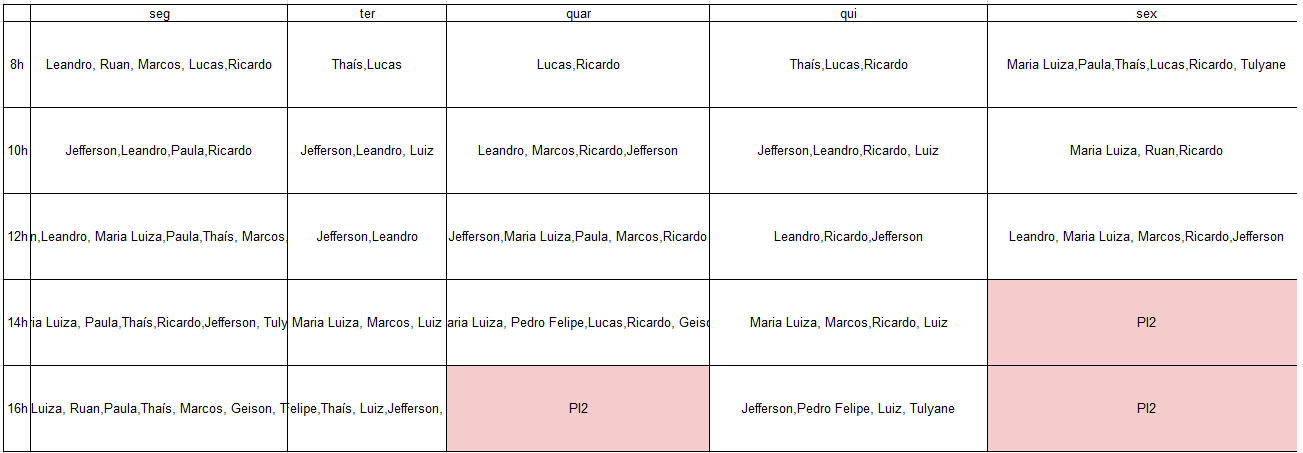
\includegraphics[scale=0.5]{figuras/horarios}
	\caption{Horários preenchidos por cada aluno se comprometendo a participar de atividades relacionadas com o projeto RoBoat.}
	\label{horarios}
\end{figure}

\section{Reuniões Online}

Escolhemos algumas ferramentas online para dar suporte ao nosso projeto.

\begin{enumerate}
	
	\item Google Drive : Para armazenar arquivos e documentos do projeto.
	\item Whatsapp : Para facilitar uma rápida comunicação com todos os integrantes do grupo.
	\item Basecamp : Para atribuir tarefas e acompanhar o desenvolvimento.
	\item Google Hangouts : Para realizar reuniões online através de vídeo conferência. 
	
\end{enumerate}